\section{Эксперементальная часть}
В данном разделе расмотрен вывод программы

На изображении \ref{fig:bbs} отображены результаты работы алгоритма BBS и мера случайности.

% TODO: \usepackage{graphicx} required
\begin{figure}[!h]
	\centering
	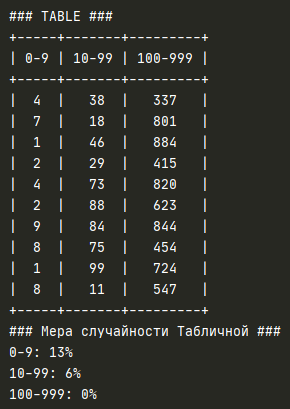
\includegraphics[width=0.7\linewidth]{src/BBS}
	\caption{Результаты BBS}
	\label{fig:bbs}
\end{figure}

На изображении \ref{fig:table} отображены табличные значения и мера случайности

% TODO: \usepackage{graphicx} required
\begin{figure}[!h]
	\centering
	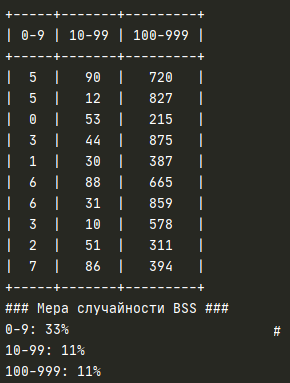
\includegraphics[width=0.7\linewidth]{src/Table}
	\caption{}
	\label{fig:table}
\end{figure}

На изображениях \ref{fig:22} и \ref{fig:23} отображена мера случайности ручного ввода.

% TODO: \usepackage{graphicx} required
\begin{figure}[!h]
	\centering
	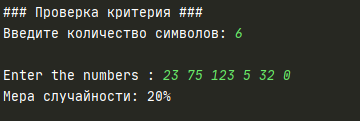
\includegraphics[width=0.7\linewidth]{src/Безымянный}
	\caption{}
	\label{fig:22}
\end{figure}

% TODO: \usepackage{graphicx} required
\begin{figure}[!h]
	\centering
	\includegraphics[width=0.7\linewidth]{"src/Мера 1"}
	\caption{}
	\label{fig:23}
\end{figure}







